%% LyX 2.1.1 created this file.  For more info, see http://www.lyx.org/.
%% Do not edit unless you really know what you are doing.
\documentclass[english]{llncs}
\usepackage[T1]{fontenc}
\usepackage[latin9]{inputenc}
\usepackage{color}
\usepackage{array}
\usepackage{url}
\usepackage{graphicx}
\PassOptionsToPackage{normalem}{ulem}
\usepackage{ulem}

\makeatletter

%%%%%%%%%%%%%%%%%%%%%%%%%%%%%% LyX specific LaTeX commands.
%% Because html converters don't know tabularnewline
\providecommand{\tabularnewline}{\\}

%%%%%%%%%%%%%%%%%%%%%%%%%%%%%% User specified LaTeX commands.
\usepackage{algorithmic}

\@ifundefined{showcaptionsetup}{}{%
 \PassOptionsToPackage{caption=false}{subfig}}
\usepackage{subfig}
\makeatother

\usepackage{babel}
\begin{document}
\title{A Study of Query Reformulation Methods for Patent Prior Art Search with Partial Patent Applications}
\maketitle
\begin{abstract}
Patents are used by entities to legally protect their inventions and
represent a multi-billion dollar industry of licensing and litigation.
In 2012, 276,788 patent applications were approved in the US alone
-- a number that has doubled in the past 15 years. While much of the
literature inspired by the evaluation framework of the CLEF-IP competition
has aimed to assist patent examiners in assessing prior art for complete
patent applications, less of this work has focused on patent search
with queries representing (partial) applications to help inventors
to assess the patentability of their ideas prior to writing a full
application. In this context, a query is much longer than in other
standard IR tasks. It can take the form of a long paragraph, or even
a very long document. This has led the research to focus on query
reformulation for patent search. Therefore, in this paper, we carry
out an intensive study and evaluation of both patent specific and
standard query reformulation methods for patent prior art search with
partial patent applications. We intend to mainly answer the following
questions: \emph{What are these query reformulation methods? How do
they work? What is the best section in a patent application to use
as a query? What is the best query reformulation method? }
\end{abstract}

\begin{keywords} Query Reformulation, Patent Search, Experimentation.
\end{keywords} 


\section{Introduction}

\noindent Patents are used by entities to legally protect their inventions
and represent a multi-billion dollar industry of licensing and litigation.
In 2012, 276,788 patent applications were approved in the US alone,
a number that has doubled in the past 15 years. Hence, helping both
inventors and patent examiners assess the patentability of a given
patent application through a patent prior art search is a critical
task.

Patent prior art search involves finding previously granted patents
that may be relevant to a new patent application. The objective and
challenges of standard formulations of patent prior art search are
different from those of standard text and web search since~\cite{Magdy2012}:
(i) queries are (partial) patent applications, which consist of documents
with hundreds of words organized into several sections, while typical
queries in text and web search constitute only a few words; (ii) patent
prior art search is a recall-oriented task, where the primary focus
is to retrieve all relevant documents at early ranks, in contrast
to text and web search that are precision-oriented, where the primary
goal is to retrieve a subset of documents that satisfy the query intent.
Another important characteristic about patent prior art search is
that, in contrast to scientific and technical writers, patent writers
tend to generalize and maximize the scope of what is protected by
a patent using a combination of abstract and specific terminology,
which make also hard to find any relevant prior work by the patent
examiner.

While much of the literature inspired by the evaluation framework
of the CLEF-IP competition has aimed to assist patent examiners in
assessing prior art for complete patent applications, less work has
focused on assessing the patentability of inventions before writing
a full patent application. Prior art search with queries that represent
unfinished patent applications is desirable, since writing a full
application is time-consuming and costly, especially if lawyers are
hired to assist.

%However prior art search with partial applications is much different than queries with a full application -- namely because the queries are much shorter and represent only parts of a patent application.

%NOTE: start a paragaph with the key idea%A patent application is organized in, at least, four sections: title,%abstract, claims and description. We assumed that a partial application%consist in one of the mentioned sections. 

\begin{figure}[!t]
\begin{centering}
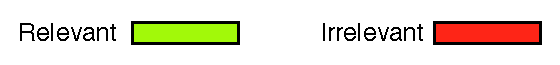
\includegraphics[width=6cm]{img/legend} 
\par\end{centering}

\begin{centering}
\subfloat[Title query.]{\begin{centering}
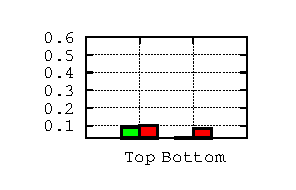
\includegraphics[width=2.9cm]{Results-CIKM2014/jaccard-qTitle-CLEF-IP2010} 
\par\end{centering}

}\subfloat[Abstract query.]{\begin{centering}
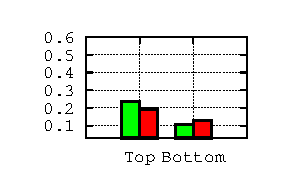
\includegraphics[width=2.9cm]{Results-CIKM2014/jaccard-qAbstract-CLEF-IP2010} 
\par\end{centering}

}\subfloat[Claims query.]{\begin{centering}
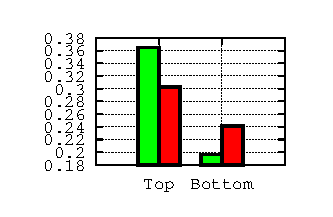
\includegraphics[width=2.9cm]{Results-CIKM2014/jaccard-qClaims-CLEF-IP2010} 
\par\end{centering}

}\subfloat[Description query.]{\begin{centering}
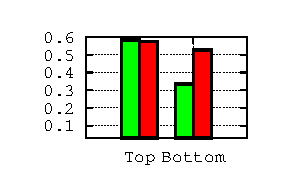
\includegraphics[width=2.9cm]{Results-CIKM2014/jaccard-qDescription-CLEF-IP2010} 
\par\end{centering}

}
\par\end{centering}

\centering{}\protect\caption{Average Jaccard similarity between fields of topics and the corresponding
(ir)relevant documents for different queries that perform the best/worst. }
{\footnotesize{}\label{fig:FailureAnalysis}}
\end{figure}


To assess the difficulty of querying with partial patent applications,
we refer to Figure~\ref{fig:FailureAnalysis}. Here we show an analysis
of the average Jaccard similarity%
\footnote{The Jaccard similarity is used to measure the term overlap between
two sets. Before applying the Jaccard similarity, patent-specific
stopwords were removed, as suggested by \cite{Mahdabi2012}.%
} between different queries (representing the title, abstract, claims,
or descriptions intended to represent a partial patent application)
and the labeled relevant (all) and irrelevant documents (top 10 irrelevant
documents ranked by BM25~\cite{Robertson1993}). We show results
for the top 100 and bottom 100 queries (100 queries that perform the
best, and 100 queries that perform the worst) of CLEP-IP 2010 evaluated
according to Mean Average Precision (MAP). Note that, while the title
section is usually composed by an average of six terms, the other
sections are longer, ranging from ten to thousands of terms. There
are three notable trends here: (i) term overlap increases from title
to description since the query size grows accordingly; (ii) the bottom
100 performing queries tend to have much smaller term overlap with
the relevant documents than the top 100 queries; and (iii) the overlap
of any relevant document set for any set of queries is less than one.

While these results suggest the description section is the best part
of a partial patent application to use as query, they also point out
that the term overlap between the queries and the relevant documents
can be very low. Also, in this context, a query is much longer than
in other standard IR tasks. It can take the form of a long paragraph
(e.g. the case of the abstract used for querying), or even a very
long document (e.g. the case of claims or the description used for
querying). This has led the research to focus on query reformulation
for patent search. Therefore, we suggest an investigation of \emph{query
reformulation} \cite{Baeza-Yates2010} methods as a means for improving
the term overlap between queries that represent partial patent applications
and relevant documents, with the objective of assessing not only the
performance of standard query reformulation methods, but also the
effectiveness of query reformulation methods that exploit patent-specific
characteristics. In summary, the contributions of this paper are the
following: 
\begin{enumerate}
\item A review of both patent specific and standard query reformulation
methods for patent prior art search with partial patent applications.
\item A thorough comparative analysis of these query reformulation methods
along several dimensions (including query type, IR model, term expansion
source, etc.) on standardized datasets of CLEF-IP. 
\end{enumerate}
The rest of the paper is organized as follows: in Section \ref{sec:QueryReformulation}
we present a number of patent specific query reformulation methods;
in Section \ref{sec:Evaluation} we present our evaluation and the
results analysis; and in Section \ref{sec:Conclusion} we conclude
with possible directions for future work.


\section{Query Reformulation for Patents}

\label{sec:QueryReformulation}

Query Reformulation is the process of transforming an initial query
$Q$ to another query $Q'$. This transformation may be either an
expansion or a reduction of the query.\emph{ Query Expansion} (QE)
\cite{Efthimiadis1996} enhances the query with additional terms likely
to occur in relevant documents. Hence, given a query representation
$Q$, QE aims to select an optimal subset $T_{k}$ of $k$ terms,
which are relevant to $Q$, then build $Q'$ such as $Q'=Q\cup T_{k}$.
As for \emph{Query Reduction} (QR) \cite{Kumaran2009}, it is the
process that reduces the query such that superfluous information is
removed. Hence, given a query representation $Q$, QR aims to select
an optimal subset $T_{k}\subset Q$ of $k$ terms, which are relevant
to $Q$, then build $Q'$ such as $Q'=T_{k}$.

In the following, in Section \ref{sec:StandardQRMethods} we first
describe standard query reformulation methods, then, in Section \ref{sec:SpecificQRMethods},
we describe few patent specific query reformulation methods.


\subsection{Standard Query Reformulation Methods}

\label{sec:StandardQRMethods}


\subsubsection{The Rocchio Algorithm for Relevance Feedback}

The Rocchio algorithm \cite{Salton1971} is a classic algorithm of
relevance feedback used mainly for query expansion. Basically, it
provides a way of incorporating relevance feedback information into
the vector space model representing a query \cite{Manning2008}. The
underlying theory behind Rocchio is to find a query vector $\overrightarrow{Q'}$,
that maximizes similarity with relevant documents while minimizing
similarity with irrelevant documents. Typically, a pseudo-relevance
feedback (PRF) set of $k$ top ranked documents obtained after an
initial run of the query is considered as the set of relevant documents
to build $\overrightarrow{Q'}$. We refer to this method as RocchioQE%
\footnote{We used the LucQE module, which provides an implementation of the
Rocchio method for Lucene. \texttt{http://lucene-qe.sourceforge.net/}%
}.

On the other hand, we can think to use Rocchio as a QR method. Basically,
the idea is once we have computed the Rocchio modified query vector,
we take only terms that appear in the initial query $Q$ and rank
them using the Rocchio score. Then, we select top $k$ terms with
the highest score to build $Q'$. We refer to this approach as RocchioQR.


\subsubsection{Maximal Marginal Relevance for Query Reformulation}

As a general method for query reformulation, we also consider a method
of ``diverse'' term selection --- an adaptation of the \emph{Maximal
Marginal Relevance} (MMR)~\cite{Carbonell1998} algorithm for result
set diversification. The idea is to use MMR for diverse term selection. 

%\subsubsection{MMR Query Expansion (MMRQE)}
%\label{sec:MMRQE}


%%%%%%%%%%%%%%%%%%%%%%%%%%%%%%%%%%%%%%%%%%%%%%%%%%%%%%%%%%%%%%%%%%%%%
\begin{figure}[!t]
\begin{centering}
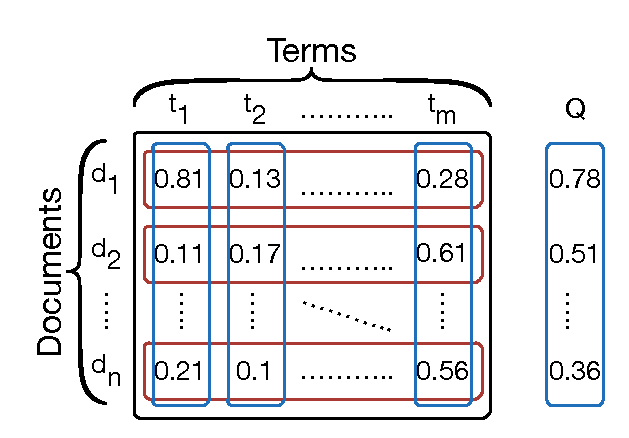
\includegraphics[width=5cm]{img/matrix} 
\par\end{centering}

\protect\caption{Notation used in MMR QE/QR.}


\label{fig:Notation} 
\end{figure}


%%%%%%%%%%%%%%%%%%%%%%%%%%%%%%%%%%%%%%%%%%%%%%%%%%%%%%%%%%%%%%%%%%%%%


In the case of query expansion, we call this method MMR Query Expansion
(MMRQE). MMRQE takes as input a PRF set, which is used to build a
document-term matrix of $n$ documents and $m$ terms as shown in
Figure~\ref{fig:Notation} (the TF-IDF is used to populate the matrix
for each document vector). To represent the query $Q$ in the documents'
dimension as in Figure~\ref{fig:Notation}, we use the BM25 or TF-IDF
score between each document $d_{i}$ and the query. Hence, given a
query representation $Q$, MMRQE aims to select an optimal subset
of $k$ terms $T_{k}^{*}\subset D$ (where $|T_{k}^{*}|=k$ and $k\ll|m|$)
relevant to $Q$ but inherently different from each other (i.e., diverse).
This can be achieved by building $T_{k}^{*}$ in a greedy manner by
choosing the next optimal term $t_{k}^{*}$ given the previous set
of optimal term selections $T_{k-1}^{*}=\{t_{1}^{*},\ldots,t_{k-1}^{*}\}$
(assuming $T_{0}^{*}=\emptyset$) using the MMR diverse selection
criterion.

Similarly, we can imagine greedily rebuild the query from scratch,
while choosing diversified terms (i.e. terms of the query). Here,
we call this approach MMR Query Reduction (MMRQR). Formally, given
a query representation $Q$, MMRQR aims to select an optimal subset
of $k$ terms $T_{k}^{*}\subset Q$ (where $|T_{k}^{*}|=k$ and $k<|Q|$)
relevant to $Q$ but inherently different from each other (i.e., diverse).
This can be achieved by building $T_{k}^{*}$ in a greedy manner by
choosing the next optimal term $t_{k}^{*}$ given the previous set
of optimal term selections $T_{k-1}^{*}=\{t_{1}^{*},\ldots,t_{k-1}^{*}\}$
(assuming $T_{0}^{*}=\emptyset$) using an adaptation of the MMR diverse
selection criterion. Note that the we use all the sections of the
patent documents in the PRF set to built the document-term matrix
of $n$ documents and $m$ terms shown in Figure~\ref{fig:Notation}.


\subsection{Patent Specific Query Reformulation Methods}

\label{sec:SpecificQRMethods}

In this section we first describe two patent specific query expansion
methods, then, we describe two patent specific query reduction methods.


\subsubsection{Synonyms Sets for Patent Query Expansion}

Magdy et al. \cite{Magdy2011} proposed a patent query expansion method,
which automatically generates candidate synonyms sets (SynSet) for
terms, and use it as a source of expansion terms. The idea for generating
the SynSet comes from the characteristics of the CLEF-IP patent collection,
where some of the sections in some patents are translated into three
languages (English, French, and German). They used these parallel
manual translations to create possible synonyms sets. Hence, for a
word $w$ in one language which has possible translations to a set
of words in another language ${w_{1},w_{2},\ldots,w_{n}}$, this set
of words can be considered as synonyms or at least related to each
other. The generated SynSet is used for query expansion in two ways:
(i) The first one use the probability associated with the SynSet entries
as a weight for each expanded term in the query (denoted WSynSet).
Therefore, each term was replaced with its SynSet entries with the
probability of each item in the SynSet acting as a weight to the term
within the query. (ii) The second one neglected this associated probability
and used uniform weighting for all synonyms of a given term (denoted
USynSet).


\subsubsection{Patent Lexicon for Query Expansion}

Mahdabi et al. \cite{Mahdabi2013} proposed to build a query-specific
patent lexicon based on definitions of the International Patent Classification
(IPC). The lexicon is simply build by removing general and patent
stop-words from the text of IPC definition pages. Each entry in the
lexicon is composed of a key and a value. The key is an IPC class
and the value is a set of terms representing the mentioned class.
Then, the lexicon build is used to extract expansion concepts related
to the context of the information need of a given query patent. To
this end, the IPC class of the query patent is searched in the lexicon
and the terms matching this class are considered as candidate expansion
terms. The approach proposed tries to combine these two complementary
vocabularies. In this paper we refer to this patent query expansion
method as IPC Codes.


\subsubsection{Language Model for Query Reduction}

In \cite{Ganguly2011}, the authors proposed a query reduction technique,
which decomposes a query (a patent section) into constituent text
segments and computes a Language Modeling (LM) similarities by calculating
the probability of generating each segment from the top ranked documents
(PRF set). Then, the query is reduced by removing the least similar
segments from the query. We refer to this method as LMQR.


\subsubsection{IPC Codes for Query Reduction}

Based on the intuition that, terms in the IPC code definition may
represent \textquotedbl{}stop-words\textquotedbl{}, especially if
they are rare (infrequent in the patent application), one can think
to reduce a patent query as follows: (i) For each patent application,
take the definitions of the IPC codes which are associated to it.
Then, (ii) rank the terms of the query according to both their frequency
in the class code definition, and their frequency in the query. Finally,
(iii) remove bottom terms of this ranking from the query (i.e. good
terms are terms that occur a lot in the query, and few in the class
code definition, whereas bad terms are those that occur few in the
query, and a lot in the class code definition). In the evaluation
section we denote this approach IPC Codes. 


\section{Experimental Evaluation}

\label{sec:Evaluation}

In this section we first explain the experiments setup for evaluating
the effectiveness of the different methods described above. Then,
we discuss the results of QE and QR methods in Sections \ref{sec:QEResults}
and \ref{sec:QRResults} respectively.


\subsection{Experimental Setup}

\label{sec:Setup}

For our experiments we used used the Lucene IR System%
\footnote{\texttt{http://lucene.apache.org/}%
} to index the English subset of CLEF-IP 2010 and CLEF-IP 2010 datasets%
\footnote{\texttt{\url{http://www.ifs.tuwien.ac.at/~clef-ip/}}%
}~\cite{Piroi2011,Roda2009} with the default stemming and stop-word
removal. We removed patent-specific stop-words as described in \cite{Magdy2012}.
CLEF-IP 2010 contains 2.6 million patent documents and CLEF-IP 2011
consists of 3 million patent documents. The English test sets of CLEF-IP
2010 and CLEF-IP 2011 correspond to 1303 and 1351 topics respectively.
In our implementation, each section of a patent (title, abstract,
claims, and description) is indexed in a separate field, so that different
sections can be used, for example, as source of expansion terms. But,
when a query is processed, all fields in the index are targeted, since
it is sensible to use all available content.

We also used the patent classification (IPC) for filtering the results
by constraining them to have common classifications with the patent
topic as suggested in previous works \cite{Lopez2009,Roda2009}. Finally,
we report MAP, and PRES, which combines Recall with the quality of
ranking and weights relevant documents lower in the ranking more highly
than MAP. We report the evaluation metrics on the top 1000 results.


\subsection{Query Expansion Results}

\label{sec:QEResults}

In this section, we discuss the results of the evaluation performed
on the QE methods described in Section \ref{sec:QueryReformulation}.
During the exploration of query expansion for patent search with partial
patent applications, there are many configuration options and associated
questions that we can consider: 
\begin{itemize}
\item \textbf{Partial patent query type:} We consider that a query of a
partial patent application consist of either the title, the abstract,
the claims or the description section. Critical questions are: what
part of a partial application an inventor should write to obtain the
best search results? and what part of a partial application suits
the best for QE?
\item \textbf{Query expansion source:} We consider the abstract, claims,
and description sections as different term sources to determine which
section offers the best source of expansion terms, e.g., are the claims
words of particularly high value as expansion terms? Note that we
consider that there is no interest to use the title as source for
the expansion since there are only few terms that we can collect from
the title field in the PRF set.
\item \textbf{Relevance model:} For initial retrieval of documents in the
\emph{pseudo-relevant} feedback set (PRF) and subsequent re-retrieval,
there are various options for the relevance ranking model. In this
work, we explore a probabilistic approach represented by the popular
BM25~\cite{Robertson1993} algorithm, as well as a vector space model
(VSM) approach, TF-IDF~\cite{Salton1975}. A natural question is
which relevance model works best for query expansion for patent prior
art search? 
\item \textbf{Term selection method:} We consider the different query expansion
methods described above, i.e. RocchioQE, MMRQE, IPC Codes, WSynSet,
USynSet. What is the best QE method for patent search?
\end{itemize}
To summarize all the results obtained over all the above configurations,
Figure \ref{fig:PRES-CLEF2010} shows the PRES obtained for all the
QE methods, while selecting the optimal number of terms used for the
expansion (number of terms that maximizes the performance for each
method). From these results, we make the following observations:
\begin{enumerate}
\item The best section to use for querying is the description section (see
Figure \ref{fig:qDescription-PRES-CLEF-IP2010}). We attribute this
to the fact that the description section has more content along with
relevant terms that define the invention since a detailed summary
of the invention is described therein.
\item The best source for query expansion is the claims section. We attribute
this to the fact that, the claims contain not only relevant, but also,
specific terminology, since the scope of the invention is described
therein. However, when querying using the claims, other sources of
query expansion provided better performance. This may be because claims
are very similar between them and contained specific terms; consequently,
the queries lack of diversity and general terms or synonyms that are
used to describe similar inventions. 
\item The description section is not either a good source for expansion,
since its content is too broad; therefore, it contains many irrelevant
terms that hurt the performance.
\item Query expansion is not useful for very long queries (i.e. description),
indicating that in advanced stages of the patent application process,
QE is not relevant. 
\item When dealing with more mid-long queries such as abstract or claims,
MMRQE is more effective than Rocchio, which suggest that diverse term
selection is not crucial for short queries. 
\item Using the IPC code definitions (as suggested by \cite{Mahdabi2013})
and SynSet (method of \cite{Magdy2011}) as a source of expansion,
gave poor performance (see IPC Codes and SynSet bars along the Figures). 
\item Finally, regarding the best term selection method, we conclude that
in general, MMRQE provides the best performance, followed by RocchioQE.
\end{enumerate}
\begin{figure*}[t]
\begin{centering}
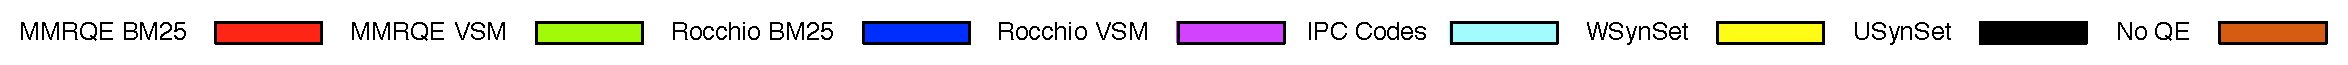
\includegraphics[width=12cm]{img/legendQE} 
\par\end{centering}

\begin{centering}
\subfloat[Query Title.]{\begin{centering}
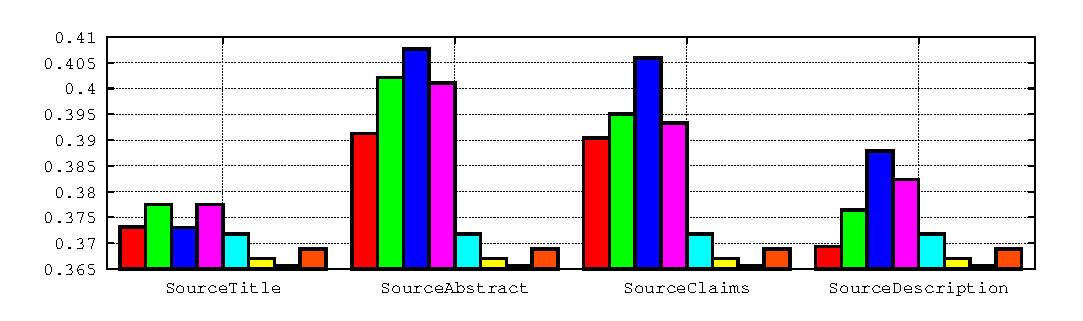
\includegraphics[width=6cm]{Results-CIKM2014/qTitle-PRES-CLEF-IP2010} 
\par\end{centering}

}\subfloat[Query Abstract.]{\begin{centering}
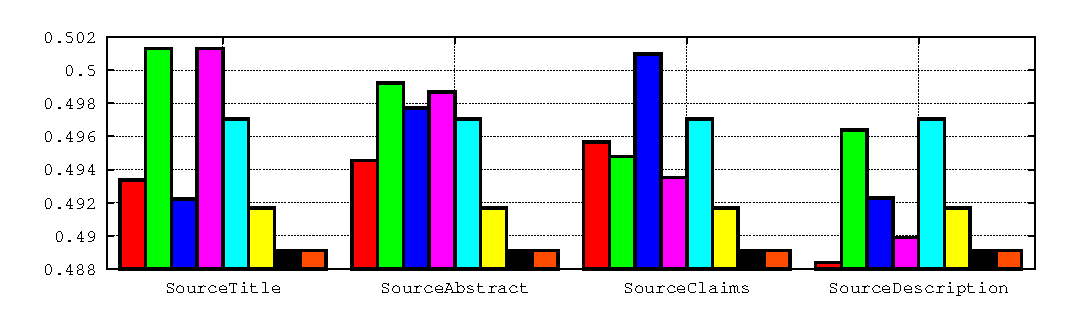
\includegraphics[width=6cm]{Results-CIKM2014/qAbstract-PRES-CLEF-IP2010} 
\par\end{centering}

}
\par\end{centering}

\begin{centering}
\subfloat[Query Claims.]{\begin{centering}
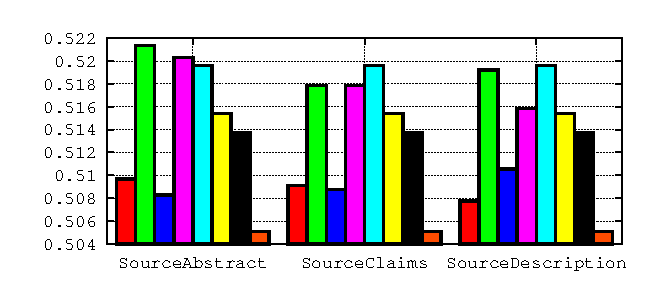
\includegraphics[width=6cm]{Results-CIKM2014/qClaims-PRES-CLEF-IP2010} 
\par\end{centering}

}\subfloat[Query Description.]{\begin{centering}
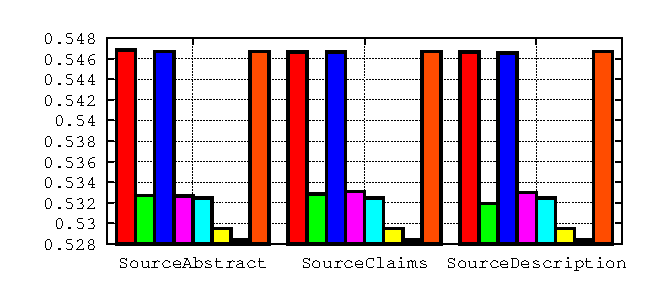
\includegraphics[width=6cm]{Results-CIKM2014/qDescription-PRES-CLEF-IP2010} 
\par\end{centering}

\label{fig:qDescription-PRES-CLEF-IP2010}}
\par\end{centering}

\protect\caption{PRES for QE methods on CLEF-IP 2010.}


\label{fig:PRES-CLEF2010} 
\end{figure*}


To give an insight of the effect of MMRQE and Rocchio over the performance,
Table \ref{tbl:QESampleQueries} shows two queries where QE methods
improved the performance. First of all, it is interesting to notice
that even if there are common terms selected to expand the queries
by both MMRQE and Rocchio, the lists of MMRQE contain more diversified
terms (at least in the first example). For the first example, relevant
patents talk about a similar idea than the application, but using
different complex and ambiguous terms. Hence, for the first query,
key terms like: \textit{rotor, blend, and suction}, were able to capture
the scope of the relevant patents to allow either retrieving them
(improving PRES), or pushing them to the top of the ranking (improving
MAP). As for the second query, MMRQE expand the query with general
terms, e.g. \textit{result, includ, extend, plural}, which probably
encourage retrieving irrelevant patents.

\begin{table*}[t]
\protect\caption{Samples of queries extracted from CLEF-IP 2011, where QE improves
the performance (P: Precision, R: Recall, AP: Average Precision, PRES:
Patent Retrieval Evaluation Score). }
\label{tbl:QESampleQueries}

\centering{}%
\begin{tabular}{|>{\raggedright}p{12cm}|}
\hline 
\textbf{\scriptsize{}1- Topic:}{\scriptsize{} EP-1921264-A2}\tabularnewline
\hline 
\textbf{\scriptsize{}Abstract:}{\scriptsize{} An article of manufacture
having a nominal profile substantially in accordance with Cartesian
coordinate values of X, Y and Z set forth...}\tabularnewline
\hline 
\begin{tabular}{>{\centering}p{12cm}}
{\scriptsize{}Baseline performance:}~{\scriptsize{}}%
\begin{tabular}{|c|c|c|c|c|c|c|c|c|c|}
\hline 
\textbf{\scriptsize{}P@5:} & {\scriptsize{}0.000} & \textbf{\scriptsize{}P@10:} & {\scriptsize{}0.000} & \textbf{\scriptsize{}R@10:} & {\scriptsize{}0.000} & \textbf{\scriptsize{}AP:} & {\scriptsize{}0.043} & \textbf{\scriptsize{}PRES:} & {\scriptsize{}0.777}\tabularnewline
\hline 
\end{tabular}\tabularnewline
\end{tabular}\tabularnewline
\hline 
\textbf{\scriptsize{}MMRQE expanded terms:}{\scriptsize{} }\textbf{\scriptsize{}\uline{airfoil}}{\scriptsize{},
}\textbf{\scriptsize{}rotor}{\scriptsize{}, }\textbf{\scriptsize{}blend}{\scriptsize{},
}\textbf{\scriptsize{}substanti}{\scriptsize{}, }\textbf{\scriptsize{}\uline{root}}{\scriptsize{},
}\textbf{\scriptsize{}\uline{portion}}{\scriptsize{}, }\textbf{\scriptsize{}includ}{\scriptsize{},
}\textbf{\scriptsize{}suction}{\scriptsize{}, }\textbf{\scriptsize{}\uline{form}}{\scriptsize{},
}\textbf{\scriptsize{}tip}\tabularnewline
\hline 
\begin{tabular}{>{\centering}p{12cm}}
{\scriptsize{}MMRQE performance:}~{\scriptsize{}}%
\begin{tabular}{|c|c|c|c|c|c|c|c|c|c|}
\hline 
\textbf{\scriptsize{}P@5:} & {\scriptsize{}0.000} & \textbf{\scriptsize{}P@10:} & {\scriptsize{}0.200} & \textbf{\scriptsize{}R@10:} & {\scriptsize{}0.666} & \textbf{\scriptsize{}AP:} & {\scriptsize{}0.124} & \textbf{\scriptsize{}PRES:} & {\scriptsize{}0.872}\tabularnewline
\hline 
\end{tabular}\tabularnewline
\end{tabular}\tabularnewline
\hline 
\textbf{\scriptsize{}Rocchio expanded terms:}\textit{\scriptsize{}
}\textbf{\scriptsize{}\uline{airfoil}}{\scriptsize{}, }{\scriptsize{}\uline{trail}}{\scriptsize{},
}{\scriptsize{}\uline{edg}}{\scriptsize{}, }{\scriptsize{}\uline{cool}}{\scriptsize{},
}\textbf{\scriptsize{}\uline{form}}{\scriptsize{}, }{\scriptsize{}\uline{blade}}{\scriptsize{},
}{\scriptsize{}\uline{side}}{\scriptsize{}, }\textbf{\scriptsize{}\uline{portion}}{\scriptsize{},
}\textbf{\scriptsize{}\uline{root}}{\scriptsize{}, }{\scriptsize{}\uline{lead}}\tabularnewline
\hline 
\begin{tabular}{>{\centering}p{12cm}}
{\scriptsize{}Rocchio performance:}~{\scriptsize{}}%
\begin{tabular}{|c|c|c|c|c|c|c|c|c|c|}
\hline 
\textbf{\scriptsize{}P@5:} & {\scriptsize{}0.000} & \textbf{\scriptsize{}P@10:} & {\scriptsize{}0.100} & \textbf{\scriptsize{}R@10:} & {\scriptsize{}0.333} & \textbf{\scriptsize{}AP:} & {\scriptsize{}0.100} & \textbf{\scriptsize{}PRES:} & {\scriptsize{}0.822}\tabularnewline
\hline 
\end{tabular}\tabularnewline
\end{tabular}\tabularnewline
\hline 
\hline 
\textbf{\scriptsize{}3- Topic: }{\scriptsize{}EP-1754935-A1}\tabularnewline
\hline 
\textbf{\scriptsize{}Abstract:}{\scriptsize{} The fire-rated recessed
downlight includes a mantle. A radiating mouth (4) is defined in the
mantle. A dilatable fireproof piece (5) is fixed in the radiating
mouth (4). Radiating apertures (6 or 6') corresponding to...}\tabularnewline
\hline 
\begin{tabular}{>{\centering}p{12cm}}
{\scriptsize{}Baseline performance:}~{\scriptsize{}}%
\begin{tabular}{|c|c|c|c|c|c|c|c|c|c|}
\hline 
\textbf{\scriptsize{}P@5:} & {\scriptsize{}0.200} & \textbf{\scriptsize{}P@10:} & {\scriptsize{}0.100} & \textbf{\scriptsize{}R@10:} & {\scriptsize{}0.111} & \textbf{\scriptsize{}AP:} & {\scriptsize{}0.086} & \textbf{\scriptsize{}PRES:} & {\scriptsize{}0.801}\tabularnewline
\hline 
\end{tabular}\tabularnewline
\end{tabular}\tabularnewline
\hline 
\textbf{\scriptsize{}MMRQE expanded terms: }\textbf{\scriptsize{}\uline{mmateri}}{\scriptsize{},
}\textbf{\scriptsize{}\uline{adapt}}{\scriptsize{}, }\textbf{\scriptsize{}\uline{2}}{\scriptsize{},
}\textbf{\scriptsize{}\uline{hous}}{\scriptsize{}, }\textbf{\scriptsize{}\uline{light}}{\scriptsize{},
}\textbf{\scriptsize{}\uline{compris}}{\scriptsize{}, }\textbf{\scriptsize{}result}{\scriptsize{},
}\textbf{\scriptsize{}\uline{form}}{\scriptsize{}, }\textbf{\scriptsize{}\uline{support}}{\scriptsize{},
}\textbf{\scriptsize{}includ}{\scriptsize{}, }\textbf{\scriptsize{}\uline{side}}{\scriptsize{},
}\textbf{\scriptsize{}\uline{mount}}{\scriptsize{}, }\textbf{\scriptsize{}\uline{4}}{\scriptsize{},
}\textbf{\scriptsize{}\uline{3}}{\scriptsize{}, }\textbf{\scriptsize{}\uline{5}}{\scriptsize{},
}\textbf{\scriptsize{}plural}{\scriptsize{}, }\textbf{\scriptsize{}fit}{\scriptsize{},
}\textbf{\scriptsize{}\uline{1}}{\scriptsize{}, }\textbf{\scriptsize{}extend}{\scriptsize{},
}\textbf{\scriptsize{}\uline{recess}}\tabularnewline
\hline 
\begin{tabular}{>{\centering}p{12cm}}
{\scriptsize{}MMRQE performance:}~{\scriptsize{}}%
\begin{tabular}{|c|c|c|c|c|c|c|c|c|c|}
\hline 
\textbf{\scriptsize{}P@5:} & {\scriptsize{}0.000} & \textbf{\scriptsize{}P@10:} & {\scriptsize{}0.100} & \textbf{\scriptsize{}R@10:} & {\scriptsize{}0.111} & \textbf{\scriptsize{}AP:} & {\scriptsize{}0.044} & \textbf{\scriptsize{}PRES:} & {\scriptsize{}0.767}\tabularnewline
\hline 
\end{tabular}\tabularnewline
\end{tabular}\tabularnewline
\hline 
\textbf{\scriptsize{}Rocchio expanded terms:}\textbf{\scriptsize{}\uline{materi}}{\scriptsize{},
}\textbf{\scriptsize{}\uline{2}}{\scriptsize{}, }\textbf{\scriptsize{}\uline{compris}}{\scriptsize{},
}\textbf{\scriptsize{}\uline{light}}{\scriptsize{}, }\textbf{\scriptsize{}\uline{adapt}}{\scriptsize{},
}\textbf{\scriptsize{}\uline{support}}{\scriptsize{}, }\textbf{\scriptsize{}\uline{form}}{\scriptsize{},
}\textbf{\scriptsize{}\uline{3}}{\scriptsize{}, }\textbf{\scriptsize{}\uline{1}}{\scriptsize{},
}{\scriptsize{}\uline{surfac}}{\scriptsize{}, }\textbf{\scriptsize{}\uline{5}}{\scriptsize{},
}\textbf{\scriptsize{}\uline{4}}{\scriptsize{}, }\textbf{\scriptsize{}\uline{side}}{\scriptsize{},
}\textbf{\scriptsize{}\uline{recess}}{\scriptsize{}, }\textbf{\scriptsize{}\uline{hous}}{\scriptsize{},
}{\scriptsize{}\uline{fire}}{\scriptsize{}, }{\scriptsize{}\uline{10}}{\scriptsize{},
}\textbf{\scriptsize{}\uline{mount}}{\scriptsize{}, }{\scriptsize{}\uline{resist}}{\scriptsize{},
}{\scriptsize{}\uline{wall}}\tabularnewline
\hline 
\begin{tabular}{>{\centering}p{12cm}}
{\scriptsize{}Rocchio performance:}~{\scriptsize{}}%
\begin{tabular}{|c|c|c|c|c|c|c|c|c|c|}
\hline 
\textbf{\scriptsize{}P@5:} & {\scriptsize{}0.400} & \textbf{\scriptsize{}P@10:} & {\scriptsize{}0.200} & \textbf{\scriptsize{}R@10:} & {\scriptsize{}0.222} & \textbf{\scriptsize{}AP:} & {\scriptsize{}0.146} & \textbf{\scriptsize{}PRES:} & {\scriptsize{}0.821}\tabularnewline
\hline 
\end{tabular}\tabularnewline
\end{tabular}\tabularnewline
\hline 
\end{tabular}
\end{table*}


\begin{figure*}[t]
\begin{centering}
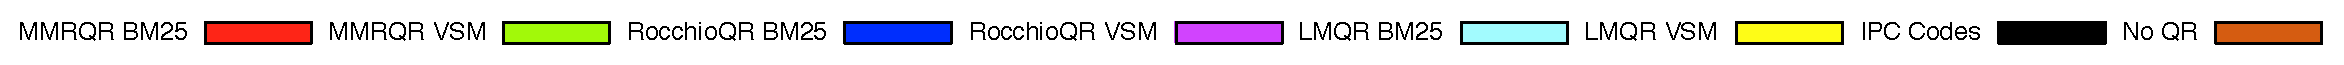
\includegraphics[width=12cm]{img/legendQR} 
\par\end{centering}

\begin{centering}
\subfloat[Query Abstract.]{\begin{centering}
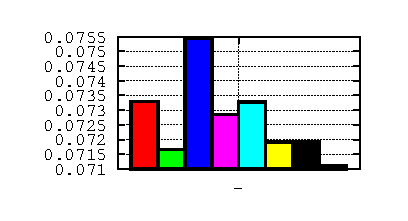
\includegraphics[width=4cm]{mmrqrResults/qAbstract-MAP-CLEF-IP2011} 
\par\end{centering}

}\subfloat[Query Claims.]{\begin{centering}
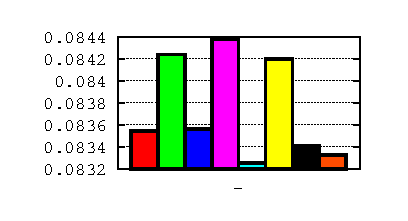
\includegraphics[width=4cm]{mmrqrResults/qClaims-MAP-CLEF-IP2011} 
\par\end{centering}

}\subfloat[Query Description.]{\begin{centering}
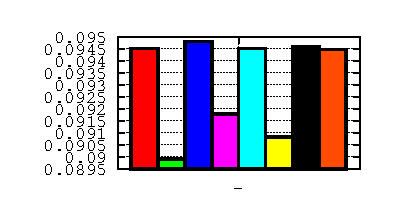
\includegraphics[width=4cm]{mmrqrResults/qDescription-MAP-CLEF-IP2011} 
\par\end{centering}

}
\par\end{centering}

\protect\caption{MAP for QR methods on CLEF-IP 2011.}


\label{fig:QR-PRES-CLEF-IP2011}
\end{figure*}


\begin{figure*}[t]
\begin{centering}
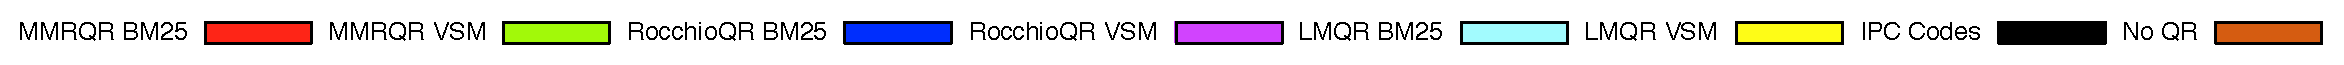
\includegraphics[width=12cm]{img/legendQR} 
\par\end{centering}

\begin{centering}
\subfloat[Query Abstract.]{\begin{centering}
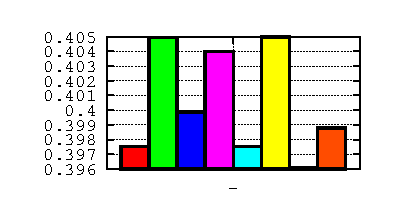
\includegraphics[width=4cm]{mmrqrResults/qAbstract-PRES-CLEF-IP2011} 
\par\end{centering}

}\subfloat[Query Claims.]{\begin{centering}
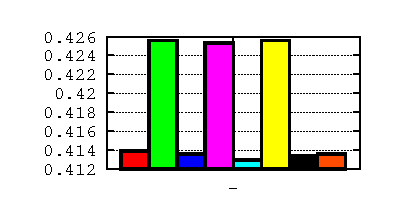
\includegraphics[width=4cm]{mmrqrResults/qClaims-PRES-CLEF-IP2011} 
\par\end{centering}

}\subfloat[Query Description.]{\begin{centering}
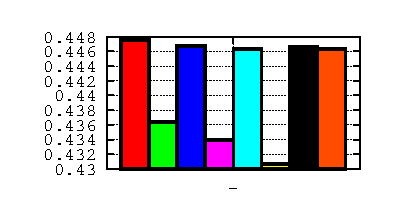
\includegraphics[width=4cm]{mmrqrResults/qDescription-PRES-CLEF-IP2011} 
\par\end{centering}

}
\par\end{centering}

\protect\caption{PRES for QR methods on CLEF 2011.}


\label{fig:QR-MAP-CLEF-IP2011} 
\end{figure*}



\subsection{Query Reduction Results}

\label{sec:QRResults}

In this section, we discuss the results of the evaluation performed
on the QR methods described in Section \ref{sec:QueryReformulation}.
Similarly, we carry out comprehensive experiments with the following
specific options and associated questions: 
\begin{itemize}
\item \textbf{Partial patent query type:} We apply QR methods to a query
of a partial patent application, which consist of the abstract, the
claims or the description sections. A critical question is what part
of a partial application suits the best for QR? Note that we consider
that there is no interest in reducing a title query since it contains
only few terms. 
\item \textbf{Term selection method:} We consider the different query reduction
methods described above, i.e. RocchioQR, MMRQR, LMQR, IPC Codes. What
is the best QR method for patent search?
\end{itemize}
To summarize all the results obtained over all the above configurations,
Figures \ref{fig:QR-PRES-CLEF-IP2011}, and \ref{fig:QR-MAP-CLEF-IP2011}
show the performance obtained for all the QR methods, when selecting
the optimal number of terms removed from the original queries (number
of terms removed that maximizes the performance for each method).
From these results, we make the following observations: 
\begin{enumerate}
\item Query reduction is often useful for mid-long queries (i.e. abstract
and claims), but not useful for very long queries since no method
outperforms the baseline (i.e. No QR). Since many confusing terms
are used in the description part, probably current QR methods failed
to distinguish useless terms to be removed. This can be an interesting
research direction to investigate for future work. 
\item Dealing with mid-long queries, VSM performs better than BM25, while
for very long query (i.e. description), BM25 based QR methods perform
better than VSM based QR methods. \textcolor{blue}{(Reda: Any suggestion
to explain that?)}
\item In general, RocchioQR and MMRQR provide better performance than the
other methods.
\end{enumerate}
To give an insight of the effect of MMRQR and RocchioQR over the performance,
Table \ref{tbl:QRSampleQueries} shows some queries where QR methods
are helpful. First, we notice that even if there is common terms removed
from the original queries by both MMRQR and RocchioQR, the lists of
MMRQR contain more similar terms (e.g. \textit{laser, light, interferometer}
for the first example). For the first example, MMRQR removed similar
terms from the queries, which favor finding more diverse patent relevant
to the patent applications. However, for the third query, MMRQR removed
the main terms from the query (\textit{motor}, and thermal \textit{load}),
which likely decrease the quality of the query.

\begin{table*}[t]
\protect\caption{Samples of queries extracted from CLEF-IP 2011, where MMRQR and RocchioQR
improve the performance. (P: Precision, R: Recall, AP: Average Precision,
PRES: Patent Retrieval Evaluation Score). }
\label{tbl:QRSampleQueries}

\centering{}%
\begin{tabular}{|>{\raggedright}p{12cm}|}
\hline 
\textbf{\scriptsize{}1- Topic: }{\scriptsize{}EP-1424597-A2}\tabularnewline
\hline 
\textbf{\scriptsize{}Abstract:}{\scriptsize{} Measurements of an interferometric
measurement system are corrected for variations of atmospheric conditions
such as pressure, temperature and turbulence using measurements from
a second harmonic interferometer (10). A ramp, representing the dependence
of...}\tabularnewline
\hline 
\begin{tabular}{>{\centering}p{12cm}}
{\scriptsize{}Baseline performance:}~{\scriptsize{}}%
\begin{tabular}{|c|c|c|c|c|c|c|c|c|c|}
\hline 
\textbf{\scriptsize{}P@5:} & {\scriptsize{}0.000} & \textbf{\scriptsize{}P@10:} & {\scriptsize{}0.000} & \textbf{\scriptsize{}R@10:} & {\scriptsize{}0.000} & \textbf{\scriptsize{}AP:} & {\scriptsize{}0.022} & \textbf{\scriptsize{}PRES:} & {\scriptsize{}0.648}\tabularnewline
\hline 
\end{tabular}\tabularnewline
\end{tabular}\tabularnewline
\hline 
\textbf{\scriptsize{}MMRQR removed terms: temperatur}{\scriptsize{},
}\textbf{\scriptsize{}detector}{\scriptsize{}, }\textbf{\scriptsize{}path}{\scriptsize{},
}\textbf{\scriptsize{}laser}{\scriptsize{}, }\textbf{\scriptsize{}light}{\scriptsize{},
}\textbf{\scriptsize{}interferometr}{\scriptsize{}, }\textbf{\scriptsize{}brewster}{\scriptsize{},
}\textbf{\scriptsize{}sensit}{\scriptsize{}, }\textbf{\scriptsize{}repres}{\scriptsize{},
}\textbf{\scriptsize{}sourc}\tabularnewline
\hline 
\begin{tabular}{>{\centering}p{12cm}}
{\scriptsize{}MMRQR performance:}~{\scriptsize{}}%
\begin{tabular}{|c|c|c|c|c|c|c|c|c|c|}
\hline 
\textbf{\scriptsize{}P@5:} & {\scriptsize{}0.000} & \textbf{\scriptsize{}P@10:} & {\scriptsize{}0.100} & \textbf{\scriptsize{}R@10:} & {\scriptsize{}0.166} & \textbf{\scriptsize{}AP:} & {\scriptsize{}0.053} & \textbf{\scriptsize{}PRES:} & {\scriptsize{}0.761}\tabularnewline
\hline 
\end{tabular}\tabularnewline
\end{tabular}\tabularnewline
\hline 
\textbf{\scriptsize{}RocchioQR removed terms: }{\scriptsize{}\uline{minim}}{\scriptsize{},
}{\scriptsize{}\uline{conduct}}{\scriptsize{}, }{\scriptsize{}\uline{variat}}{\scriptsize{},
}{\scriptsize{}\uline{shi}}{\scriptsize{}, }{\scriptsize{}\uline{turbul}}{\scriptsize{},
}{\scriptsize{}\uline{condit}}{\scriptsize{}, }{\scriptsize{}\uline{pressur}}{\scriptsize{},
}{\scriptsize{}\uline{remov}}{\scriptsize{}, }{\scriptsize{}\uline{ramp}}{\scriptsize{},
}{\scriptsize{}\uline{thick}}\tabularnewline
\hline 
\begin{tabular}{>{\centering}p{12cm}}
{\scriptsize{}RocchioQR performance:}~{\scriptsize{}}%
\begin{tabular}{|c|c|c|c|c|c|c|c|c|c|}
\hline 
\textbf{\scriptsize{}P@5:} & {\scriptsize{}0.000} & \textbf{\scriptsize{}P@10:} & {\scriptsize{}0.000} & \textbf{\scriptsize{}R@10:} & {\scriptsize{}0.000} & \textbf{\scriptsize{}AP:} & {\scriptsize{}0.036} & \textbf{\scriptsize{}PRES:} & {\scriptsize{}0.724}\tabularnewline
\hline 
\end{tabular}\tabularnewline
\end{tabular}\tabularnewline
\hline 
\hline 
\textbf{\scriptsize{}3- Topic: }{\scriptsize{}EP-1314594-A1}\tabularnewline
\hline 
\textbf{\scriptsize{}Abstract:}{\scriptsize{} An air conditioner for
air conditioning the interior of a compartment includes a compressor
(C) and an electric motor (84). The compressor (C) compresses refrigerant...}\tabularnewline
\hline 
\begin{tabular}{>{\centering}p{12cm}}
{\scriptsize{}Baseline performance:}~{\scriptsize{}}%
\begin{tabular}{|c|c|c|c|c|c|c|c|c|c|}
\hline 
\textbf{\scriptsize{}P@5:} & {\scriptsize{}0.600} & \textbf{\scriptsize{}P@10:} & {\scriptsize{}0.400} & \textbf{\scriptsize{}R@10:} & {\scriptsize{}0.307} & \textbf{\scriptsize{}AP:} & {\scriptsize{}0.301} & \textbf{\scriptsize{}PRES:} & {\scriptsize{}0.777}\tabularnewline
\hline 
\end{tabular}\tabularnewline
\end{tabular}\tabularnewline
\hline 
\textbf{\scriptsize{}MMRQR removed terms:}{\scriptsize{} }\textbf{\scriptsize{}\uline{refer}}{\scriptsize{},
}\textbf{\scriptsize{}motor}{\scriptsize{}, }\textbf{\scriptsize{}\uline{current}}{\scriptsize{},
}\textbf{\scriptsize{}\uline{relat}}{\scriptsize{}, }\textbf{\scriptsize{}condit}{\scriptsize{},
}\textbf{\scriptsize{}constant}{\scriptsize{}, }\textbf{\scriptsize{}\uline{suppli}}{\scriptsize{},
}\textbf{\scriptsize{}\uline{compress}}{\scriptsize{}, }\textbf{\scriptsize{}load}{\scriptsize{},
}\textbf{\scriptsize{}\uline{match}}\tabularnewline
\hline 
\begin{tabular}{>{\centering}p{12cm}}
{\scriptsize{}MMRQR performance:}~{\scriptsize{}}%
\begin{tabular}{|c|c|c|c|c|c|c|c|c|c|}
\hline 
\textbf{\scriptsize{}P@5:} & {\scriptsize{}0.400} & \textbf{\scriptsize{}P@10:} & {\scriptsize{}0.500} & \textbf{\scriptsize{}R@10:} & {\scriptsize{}0.384} & \textbf{\scriptsize{}AP:} & {\scriptsize{}0.221} & \textbf{\scriptsize{}PRES:} & {\scriptsize{}0.774}\tabularnewline
\hline 
\end{tabular}\tabularnewline
\end{tabular}\tabularnewline
\hline 
\textbf{\scriptsize{}RocchioQR removed terms: }{\scriptsize{}\uline{compart}}{\scriptsize{},
}\textbf{\scriptsize{}\uline{suppli}}{\scriptsize{}, }\textbf{\scriptsize{}\uline{current}}{\scriptsize{},
}{\scriptsize{}\uline{ga}}{\scriptsize{}, }\textbf{\scriptsize{}\uline{refer}}{\scriptsize{},
}\textbf{\scriptsize{}\uline{compress}}{\scriptsize{}, }\textbf{\scriptsize{}\uline{relat}}{\scriptsize{},
}{\scriptsize{}\uline{interior}}{\scriptsize{}, }{\scriptsize{}\uline{thermal}}{\scriptsize{},
}\textbf{\scriptsize{}\uline{match}}{\scriptsize{}, }\tabularnewline
\hline 
\begin{tabular}{>{\centering}p{12cm}}
{\scriptsize{}RocchioQR performance:}~{\scriptsize{}}%
\begin{tabular}{|c|c|c|c|c|c|c|c|c|c|}
\hline 
\textbf{\scriptsize{}P@5:} & {\scriptsize{}0.400} & \textbf{\scriptsize{}P@10:} & {\scriptsize{}0.400} & \textbf{\scriptsize{}R@10:} & {\scriptsize{}0.307} & \textbf{\scriptsize{}AP:} & {\scriptsize{}0.266} & \textbf{\scriptsize{}PRES:} & {\scriptsize{}0.802}\tabularnewline
\hline 
\end{tabular}\tabularnewline
\end{tabular}\tabularnewline
\hline 
\end{tabular}
\end{table*}



\section{Conclusion and Future Work}

\label{sec:Conclusion}

In this paper we analyzed general and specific query reformulation
methods for patent prior art search with partial (incomplete) patent
applications on patent retrieval corpuses of CLEF-IP. We demonstrated
that QE methods are critical for short queries, i.e. title, abstract,
and claims, but useless for very long queries, i.e. the description
section. We also showed that the description is the best section that
works with QE to query with, followed by the claims, the abstract,
then the title section. As for the source of query expansion terms,
the claims seems to be the best section since it provides terms and
terminology specific to the patent application domain. In the same
vein, we also found that the patent specific fields are more suited
as a source for expansion than external sources such as synonym dictionaries,
or IPC codes. For QE, future work concerns how can we exploit patent
specific meta-data such as inventor and citation networks to retrieve
more relevant terms to the query.

Regarding QR methods, we showed that these techniques are effective
to some extent especially for the abstract and claims sections, which
are considered as mid-long sections in a patent application. The improvement
of QR method on the description section is not that significant. Future
work may consist of exploiting query quality predictors to identify
useless terms in a query using machine learning methods.

Finally, it is clear that for a patent examiner, using the description
section of a patent application with perhaps a QR method like MMRQR
or RocchioQR will help to find the most relevant documents (to invalidate
the application). However, for inventors, before investing too much
time in writing a full patent application, we believe that it's better
to first write a brief description of their invention in the form
of an abstract. Then, use Rocchio with expanded terms coming from
the claims to get the most relevant documents to make a prior art
search task (to position the current invention with related work).

{\scriptsize{} \bibliographystyle{abbrv}
\bibliography{biblio}
}
\end{document}
